\chapter{\ifproject%
      \ifenglish Project Structure and Methodology\else โครงสร้างและขั้นตอนการทำงาน\fi
  \else%
      \ifenglish Project Structure\else โครงสร้างของโครงงาน\fi
  \fi
 }

ในบทนี้จะกล่าวถึงหลักการ และการออกแบบระบบ

\makeatletter

% \renewcommand\section{\@startsection {section}{1}{\z@}%
%                                    {13.5ex \@plus -1ex \@minus -.2ex}%
%                                    {2.3ex \@plus.2ex}%
%                                    {\normalfont\large\bfseries}}

\makeatother
%\vspace{2ex}
% \titleformat{\section}{\normalfont\bfseries}{\thesection}{1em}{}
% \titlespacing*{\section}{0pt}{10ex}{0pt}

\section{หลักการทำงานของระบบ}


% \begin{figure}
% \begin{center}
% \includegraphics{800px-Briny_Beach.jpg}
% \end{center}
% \caption[Poem]{The Walrus and the Carpenter}
% \label{fig:walrus}
% \end{figure}

\subsection{ภาพรวมของระบบ (System Overview)}
\begin{figure}[h]
    \begin{center}
        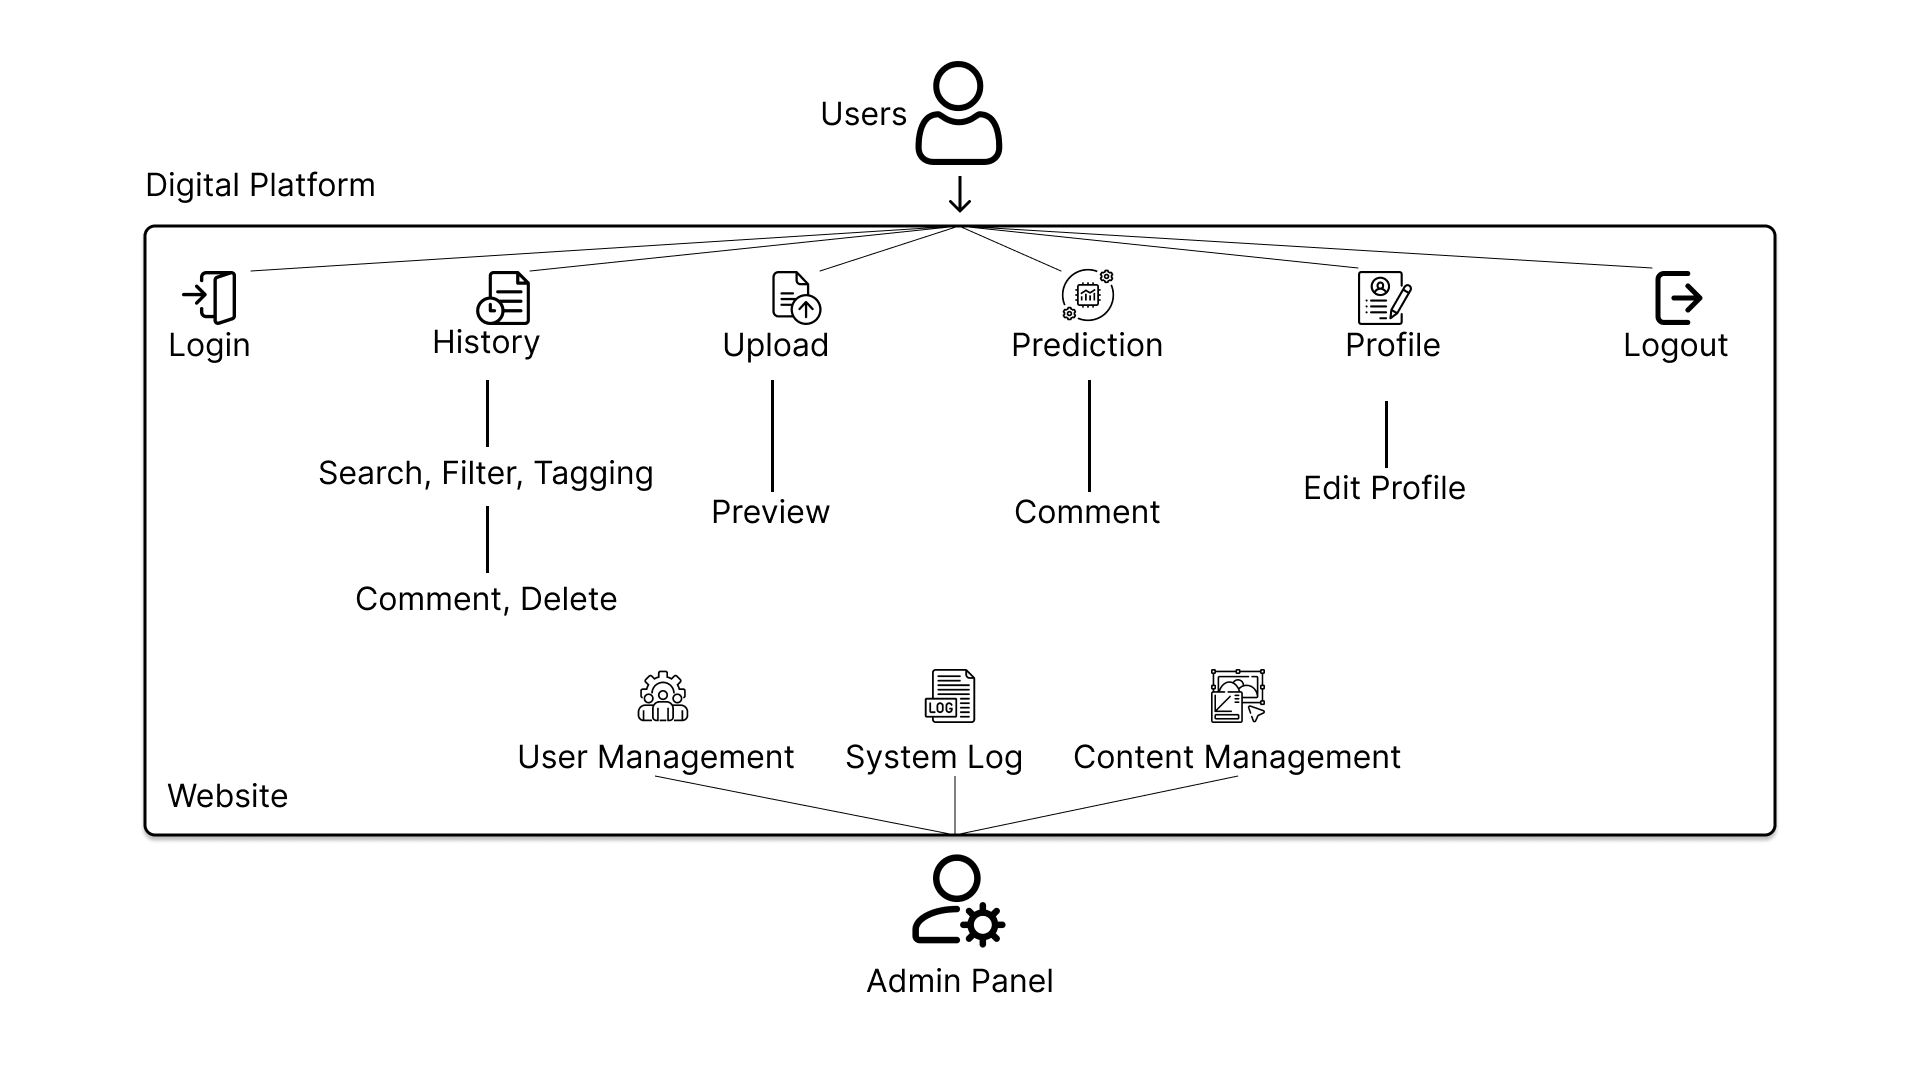
\includegraphics[width=1\textwidth]{img/Overview System Design.png}
    \end{center}
    \caption[Poem]{System Overview}
    \label{fig:walrus}
\end{figure}

ภาพรวมการทำงานของระบบนี้ จะมีส่วนการทำงานหลัก ๆ ดังนี้
\begin{itemize}
    \item ระบบการอัพโหลดและการทำนายรอยโรคในช่องปากโดย AI
    \item ระบบประวัติการอัพโหลดและการทำนายรอยโรคในช่องปากสำหรับแต่ละผู้ใช้งาน
    \item ระบบการวงรอยโรคสำหรับทันตแพทย์ (Annotation)
    \item ระบบการแพทย์ทางไกล (Telemedicine) สำหรับให้ความคิดเห็นระหว่างทันตแพทย์ผู้เชี่ยวชาญกับทันตแพทย์ทั่วไป, อาสาสมัครสาธารณสุขประจำหมู่บ้าน, ทันตบุคลากรและผู้ใช้ทั่วไป
    \item ระบบจัดการผู้ใช้งาน (User Management) และระบบติดตามผู้ใช้งาน (User Tracking)
    \item ระบบจัดการข้อมูล (Data Management)
\end{itemize}

\subsubsection{ระบบการอัพโหลดและการทำนายรอยโรคในช่องปากโดย AI}


\subsubsection{ระบบการวงรอยโรคสำหรับทันตแพทย์ (Annotation)}

\subsubsection{ระบบ Tagging รอยโรคในช่องปาก}

\subsubsection{ระบบการแพทย์ทางไกล (Telemedicine)}



\subsection{โครงสร้างฐานข้อมูล (Database Schema)}
\begin{figure}[h]
    \begin{center}
        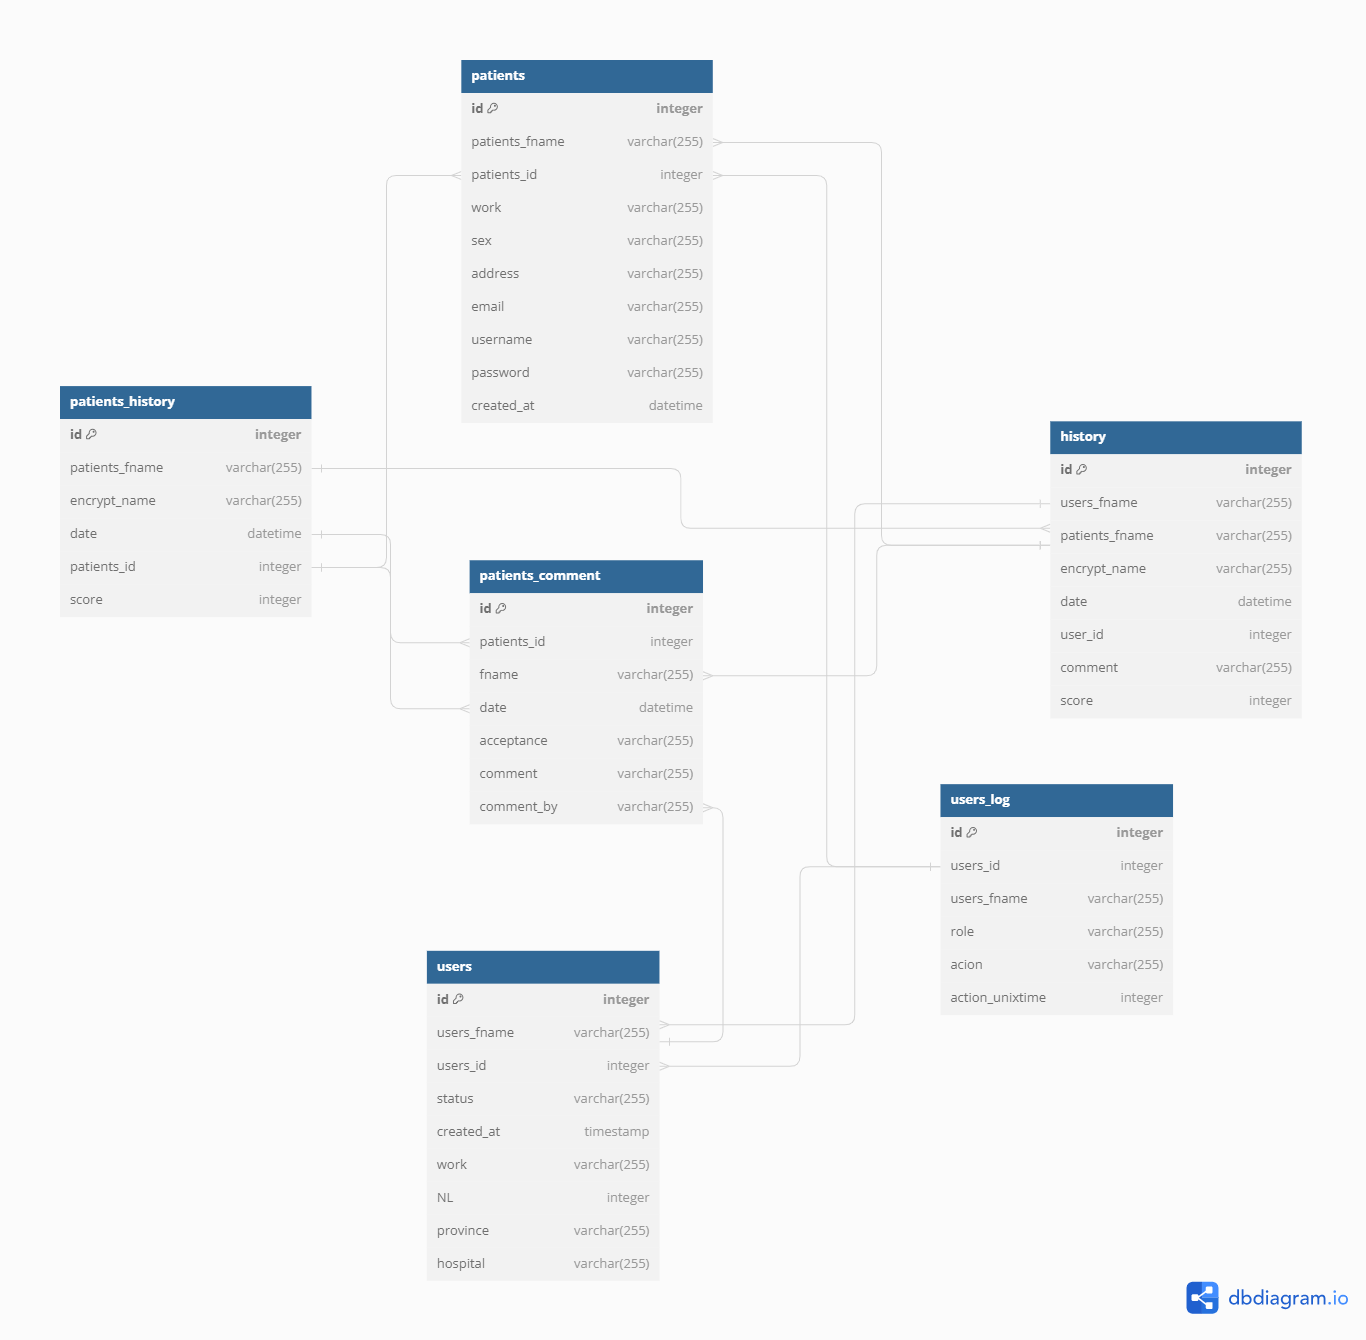
\includegraphics[width=0.9\textwidth]{img/database.png}
    \end{center}
    \caption[Poem]{Database Schema}
    \label{fig:data_schema}
\end{figure}
จากรูปที่ \ref{fig:data_schema} จะเป็นโครงสร้างของฐานข้อมูลที่ใช้ในระบบ โดยมีรายละเอียดดังนี้



Database diagram ของระบบของเรา ได้ทำการเเบ่งผู้ใช้งานเป็น 2 ส่วนหลัก ๆ คือ patients เเละ users โดย patients คือ คนไข้ทั่วไป เเละ users คือกลุ่มทันตเเพทย์ พนักงานสาธารณสุขเเละผู้ดูแลระบบ รวมถึงอสม.

ตาราง comment ระบบจะให้เฉพาะทันตเเพทย์ที่มีใบ NL ในการ comment ข้อมูลเท่านั้น โดยสามารถบอกได้ว่าเห็นด้วยหรือไม่เห็นด้วย ด้วยเหตุผลอย่างไร 

ตาราง \texttt{users\_log} เป็น table ที่สามารถดูได้เฉพาะ user ที่เป็นผู้ดูแลระบบเท่านั้น 
โดยจะบอกเกี่ยวกับ action ของผู้ใช้งานทุกคนว่า ได้มี interact กับระบบอย่างไรบ้าง โดยที่ action จะมี login, logout , delete รวมถึว action ที่สำคัญต่าง ๆ ไม่ว่าจะเป็น delete user, การ uplaod image โดยเก็บเป็น unixtime เพื่อ ทำให้ง่ายต่อการ parse

การเข้ารหัสข้อมูล (Encryption) เนื่องจากระบบของเรามีข้อมูลส่วนตัวมากมายที่เก็บเอาไว้ เราจึงต้องทำการเข้ารหัสข้อมูลตาม requirement ที่เราได้รับมา โดยจะมี file รูปภาพที่เป็นความลับของคนไข้เเละทำการเข้ารหัส password เพื่อความปลอดภัย

\section{User Interface}
ใส่ภาพหน้าจอของระบบ และอธิบาย